\documentclass[conference]{IEEEtran}
\IEEEoverridecommandlockouts
% The preceding line is only needed to identify funding in the first footnote. If that is unneeded, please comment it out.
\usepackage{cite}
\usepackage{amsmath,amssymb,amsfonts}
\usepackage{algorithmic}
\usepackage{graphicx}
\usepackage{textcomp}
\usepackage{xcolor}
\usepackage{hyperref}
\usepackage{caption}
\usepackage{subcaption}

\def\BibTeX{{\rm B\kern-.05em{\sc i\kern-.025em b}\kern-.08em
    T\kern-.1667em\lower.7ex\hbox{E}\kern-.125emX}}

\begin{document}

\title{Degradable Objects : An Application To A Distributed Data Store}

\author{\IEEEauthorblockN{Adam CHADER}
\IEEEauthorblockA{\textit{PDS track, Master of Computer Science} \\
\textit{Institut Polytechnique de Paris}\\
Palaiseau, France \\
adam.chader@telecom-paris.fr}
}

\maketitle

\begin{abstract}
Ceci est un abstract
\end{abstract}

\begin{IEEEkeywords}
Concurrent programming, parallel programming, performance, databases
\end{IEEEkeywords}

\section{Introduction}
This paper is the report of a research project realised for the Parallel And Distributed Systems master at \textit{Institut Polytechnique de Paris}. It describes the work that I realised to apply degradable data structures to Apache Ignite \cite{ignite}, a distributed data store, to improve its performance and scalability.

\subsection{Context}
Up until the begnining of the 21\textsuperscript{st} Century, there was a simple rule that could be used to predict the performances of computers. This is known as Moore's Law (Fig.~\ref{moore}). This law states that every two year, the number of transistors would double on chips. This rule could be used quite flawlessly to predict the speed of software, as there is a direct correlation between the speed of sequential programs and the frequency of CPUs. However, in recent years, several issues have surfaced regarding these assumptions : Firstly, we seem to have reached the minimum physical size of a transistor at around 5 nanometer ; secondly, the frequency that can be reached by craming all these transistors in a single CPU core is too high to be dissipated by current means \cite{moore}. As of today, it is extremely complicated and costly to significantly increase the clock speed of a single core. The solution that was found is to put multiple CPU cores in a single machine. The total number of clock cycle per second should continue increasing, while the heat would remain manageable. Intuitively, this solution is perfect : by having two cores instead of one, we could double the total frequency of the CPU, and thus double the speed of software. This is what we call \textit{linear scalability}, and it is still just a dream. There are many reason as to why it is impossible to achieve linear scalability, but they all boil down to the same issue : in order to make the most out of several CPU cores, we need to have them working at the same time. It is possible when the tasks are perfectly parallelisable, but this almost never happens when we want the cores working together. Programs need to access variables in memory, and accessing them in parallel can cause conflicts (we will explain these conflicts in detail later), they also need to aces IO which can cause an issue. The resulting effect of these issues is that parallel programs often contain sequential portions, where each core has to wait for one core to finish a task. The more sequential portions a parallel program contains, the slower the speedup is. This is described by Amdahl's Law \cite{amdahl} (Fig.~\ref{amdahl}). It describes the speedup of parallelisation as a function of the amount of sequential code.

\begin{figure}[!ht]
\centerline{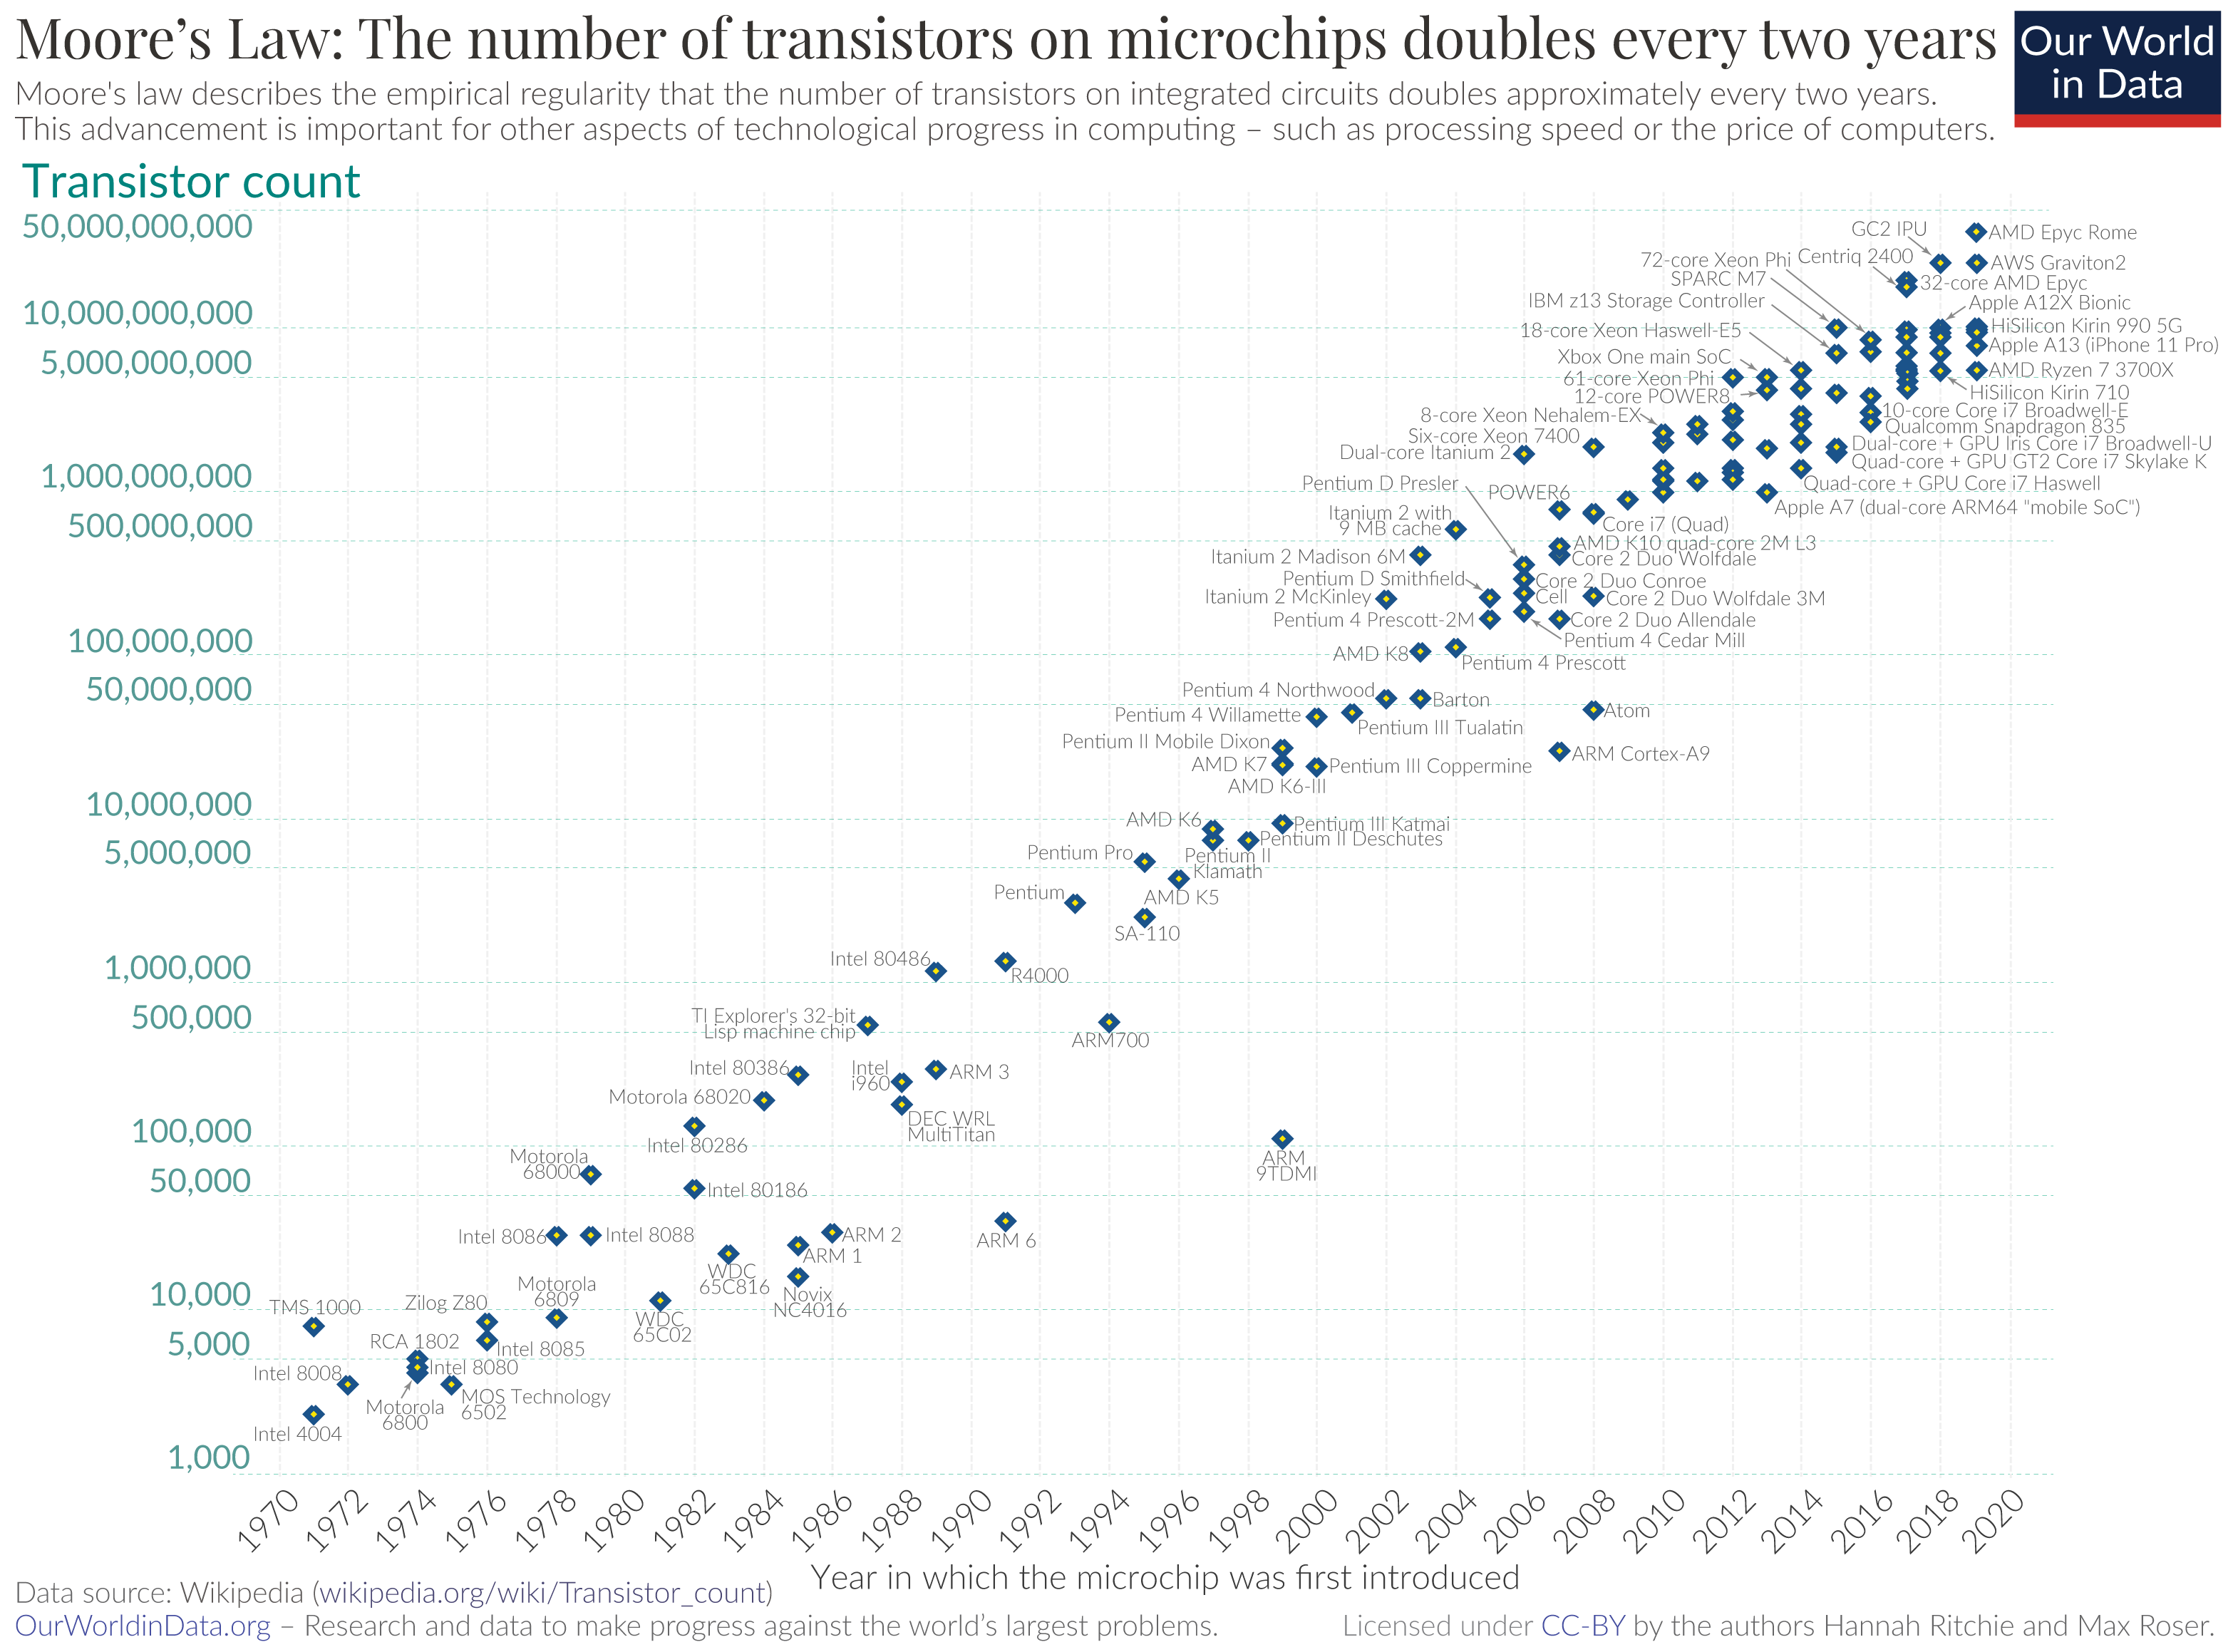
\includegraphics[width=50mm]{moore.png}}
\caption{Moore's Law.}
\label{moore}
\end{figure}

\begin{figure}[!ht]
\centerline{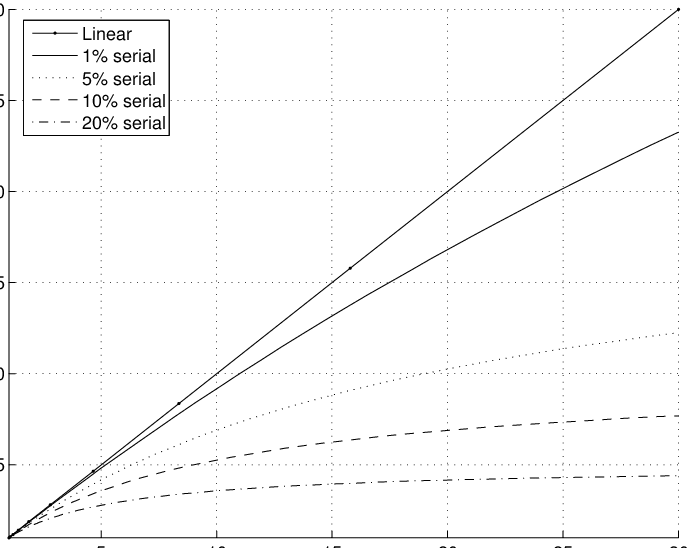
\includegraphics[width=50mm]{amdahl.png}}
\caption{Amdahl's Law}
\label{amdahl}
\end{figure}

With all this in mind, it becomes clear that the burden of increasing the performances of software no longer lies in the hand of hardware manufacturers, but rather on the hands of software engineers, who should attempt to have as little sequential code as they can in their programs.
Historically, it was the responsibility of the end programmer to parallelise their program. But there has been work to hide this work in the lower levels of the software stack \cite{scalable}, to make the shift from sequential to parrallel transparent to the higher levels. The scope of this work is at a lower level. The goal is to provide perfectly linearly scalable implementations of classic data structures, keeping the exact same interfaces, such that there could be virtually no modification to applications' source, while achieving the scalability that we desire.



\section{Conflicts and Scalability}

\section{Degradable Data Structures}

\section{Performance Analysis of Apache Ignite}

\section{Performance Evaluation}


\begin{thebibliography}{00}
\bibitem{scalable} \href{https://dl.acm.org/doi/10.1145/2699681}{Austin T. Clements, M. Frans Kaashoek, Nickolai Zeldovich, Robert T. Morris, and Eddie Kohler. 2015. The scalable commutativity rule: Designing scalable software for multicore processors. ACM Trans. Comput. Syst. 32, 4, Article 10 (January 2015), 47 pages.}
\bibitem{ignite} \href{https://ignite.apache.org/docs/latest/}{Apache Ignite}
\bibitem{gcpcompute} \href{https://cloud.google.com/compute/docs}{Google Cloud Platform Compute Engine}
\bibitem{moore} \href{https://ieeexplore.ieee.org/document/591665}{R. R. Schaller, "Moore's law: past, present and future," in IEEE Spectrum, vol. 34, no. 6, pp. 52-59, June 1997, doi: 10.1109/6.591665.}
\bibitem{amdahl} \href{https://conservancy.umn.edu/handle/11299/104341}{Gene M. Amdahl (1989), Oral history interview with Gene M. Amdahl, Charles Babbage Institute, University of Minnesota, hdl:11299/104341.}

\end{thebibliography}

\vspace{12pt}
\end{document}
